
\section{Opis baze podataka}
Informacioni sistem  restorana osmišljen je tako da umnogome olakša poslovanje samog restorana, rad zaposlenih u njemu kao i komunikaciju izmedju zaposlenih. Jedan od najbitnijih aspekata ovog informacionog si\-stema je upravo baza podataka. Pravilno dizajnirana baza podataka pruža njegovim korisnicima pristup ažuriranim, tačnim informacijama. \\
\indent Baza podataka je projektovana tako da pokriva sve slučajeve upotrebe informacionog sistema. \\
\indent U bazi postoji apstraktni tip eniteta \textbf{Osoba} iz kog su izvedeni tipovi entiteta  \textbf{Zaposleni} i \textbf{Korisnik} koji opisuju redom skup zaposlenih u restoranu i skup registrovanih korisnika restorana, tim redom. \\

Tabela \textbf{Osoba} sadrži zajedničke informacije za zaposlene i korisnike. Polje "id\_osobe" se odnosi na jedinstveno korisničko ime, a "aktivan" označava da li je zaposleni korisnik trenutno aktivan (bit 1) na nalogu restorana ili ne (bit 0). \\

\indent Registracijom korisnika na sajtu restorana dodaje se red u tabeli \textbf{Oso\-ba}. Apstraktni entitet \textbf{Osoba} se specijalizuje entitetom \textbf{Korisnik} i tabela \textbf{Korisnik} se popunjava odgovarajućim redom. \\

Slično, kreiranjem naloga za novog radnika se apstraktni entitet \textbf{Osoba} specijalizuje entitetom \textbf{Zaposleni} i tabela \textbf{Zaposleni} se popunjava odgovarajućim redom. Ova tabela povezana je sa tabelom \textbf{Uloga} ključem koji ukazuje na odgovarajuću poziciju u sistemu zaposlenih.\\

Deaktivacija naloga otpuštenog radnika vrši se samo promenom bita sa 1 na 0 u polju "aktivan" tabele \textbf{Osoba}.\\

Svaki korisnik ima pravo da ostavi utisak o kvalitetu usluge restorana. Ocenjvanje usluge restorana vrši se na osnovu polja "Jeloid\_jela" u tabeli \textbf{Ocena}. To je ujedno i strani kluč koji se odnosi na tabelu \textbf{Jelo}. Polje "vrednost" ukazuje na ocenu, a komentar nije obavezan. Tabela \textbf{Ocena} je povezana stranim ključem "KorisnikOsobaid\_osobe" i sa tabelom \textbf{Korisnik}. \\

Prilikom naručivanja (onlajn ili telefonom) dodaje se novi red u tabeli \textbf{Porudžbina} pod uslovom da je porudžbina prihvaćena. Takodje, u tabeli se bele\v zi i da li je u pitanju ketering ili ne (kolona "ketering"). Tabela je povezana sa tabelom \textbf{Korisnik} identifikatorom osobe kao i sa tabelom \textbf{Spisak} identifikatorom porudžbine. Da bi se proverila mogućnost realizacije porudžbine, dodaje se najpre novi red u tabeli \textbf{Spisak} sa traženim zahtevima. Koordinator proverava preko identifikatora jela i namirnica da li ima dovoljno zaliha trenutno u magacinu. Identifikatori jela i namirnica su povezani tabelom \textbf{Priprema}. Napomena: identifikator jela se odnosi kako na hranu, tako i na piće.
\\

U toku realizacije porud\v zbine, sve neophodne namirnice za pripremu naru\v cenog jela, koje nedostaju u kuhinji, magacioner donosi kuvaru. Dono\v senje svih tih namirnica prouzrokuje a\v zuriranje kolone "kvantitet" u tabeli \textbf{Namirnice}. Za svaku namirnicu pojedina\v cno se imanjuje njen kvantitet u magacinu.\\

\indent Kad kuvar zavr\v si pripremu bilo kog jela sa dobijenog spiska, on o tome obavesti koordinatora. Pritom se a\v zurira kolona "pripremljeno" u tabeli \textbf{Spisak} za to jelo (postavlja se na 1). Kada su sva jela sa spiska porud\v zbine pripremljena, ukoliko je data porud\v zbina u vidu keteringa, kuvar obave\v stava koordinatora, a ovaj dekoratera da je sve spremno za dekoraciju. Nakon zavr\v sene dekoracije, porud\v zbina je spremna za dostavu i o tome je, naravno, obave\v sten koordinator. To se u bazi evidentira tako \v sto se kolona "pripre\-mljena" u tabeli \textbf{Porud\v zbina} postavi na 1 za datu porud\v zbinu.\\

\indent Pripremljenu porud\v zbinu koju je zahtevao korisnik isporu\v cuje dostavlja\v c. Tom prilikom se kreira novi red u tabeli \textbf{Dostava}. Ova tabela sadr\v zi podatke o porud\v zbini, preko stranog kljuca "Porudzbinaid\_porudzbine" na tabelu \textbf{Porud\v zbina}, zatim o zaposlenom (dostavlja\v cu) preko stranog klju\v ca "ZaposleniOsobaid\_osobe" na tabelu  \textbf{Zaposleni}, kao i informacije o vremenu polaska, vremenu dostave i o tome da li je dostava uspe\v sno realizovana ili nije. Primarni klju\v c je par: id\_porudzbine, id\_osobe.\\
\indent Dostava je uspe\v sno realizovana ukoliko je dostavljena datom korisniku (kolona "uspesna" u tabeli \textbf{Dostava} se postavlja na 1).\\

Zaposleni ima pravo da podnese zahtev za odmorom ili neplacenim odustvom. Svaki ovaj zahtev implicira unošenje novog reda u tabelu \textbf{Zahtev za odsustvom}. Ova tabela jedinstveno je odredjena identifikatorom odsustva i korisničkim imenog zaposlenog i ujedno je stranim kljucem povezana sa tabelom Zaposleni. Zaposleni podnosi zahtev za neplacenim odmorom u slučaju da nema više slobodnih dana, i u tom slučaju polje "plaćeno" u odgovarajućem redu tabele biće 0. U suprotnom, tj. ukoliko zaposleni može podneti zahtev za odmorom, polje  "plaćeno" imaće vrednost 1. \\
\indent U zavisnosti od toga da li je zahtev radnika za odsustvom ili odmorom prihvaćen ili odbijen, polje "odobreno" imaće vrednost 1 ili 0. \\

Tabela \textbf{Namirnice} sadrži osnovne informacije o namirnicama u magacinu. Zaposleni magacioner vodi računa o zalihama namirnica i na osnovu podataka u ovoj tabeli zna kada i kojim namirnicama treba snabdeti magacin. \\ 
\indent Ova tabela kao primarni ključ ima kolonu "id\_namirnice". Kolona "količina" čuva podatak o količini  jednog pakovanja dotične namirnice, a kolona "merna\_jedinica"
u skladu s tim, kojom mernom jedinicom se mere pakovanja. Kolona "kvantitet" prikazuje brojno stanje pakovanja te namirnice.
Kada polje "kvantitet" ima vrednost manju od polja "minimum" u tabeli \textbf{Namirnice} u redu čiji je identifikator id\_namirnice baš te namirnice, magacioner zna da je ta namirnica na isteku svojih zaliha i da ju je potrebno naručiti. \\
\indent Kako se menja stanje namirnice u magacinu tako se ažurira i polje "kvantitet" i postavlja na vrednost trenutnog stanja te namirnice u maga\-cinu.
\href{https://raw.githubusercontent.com/JelenaCosic1994/Porucivanje_hrane/master/slike/Baza.jpg}{Ovde} se nalazi slika veće rezolucije.

\begin{figure}[!h]
    \leavevmode
    \begin{center}
    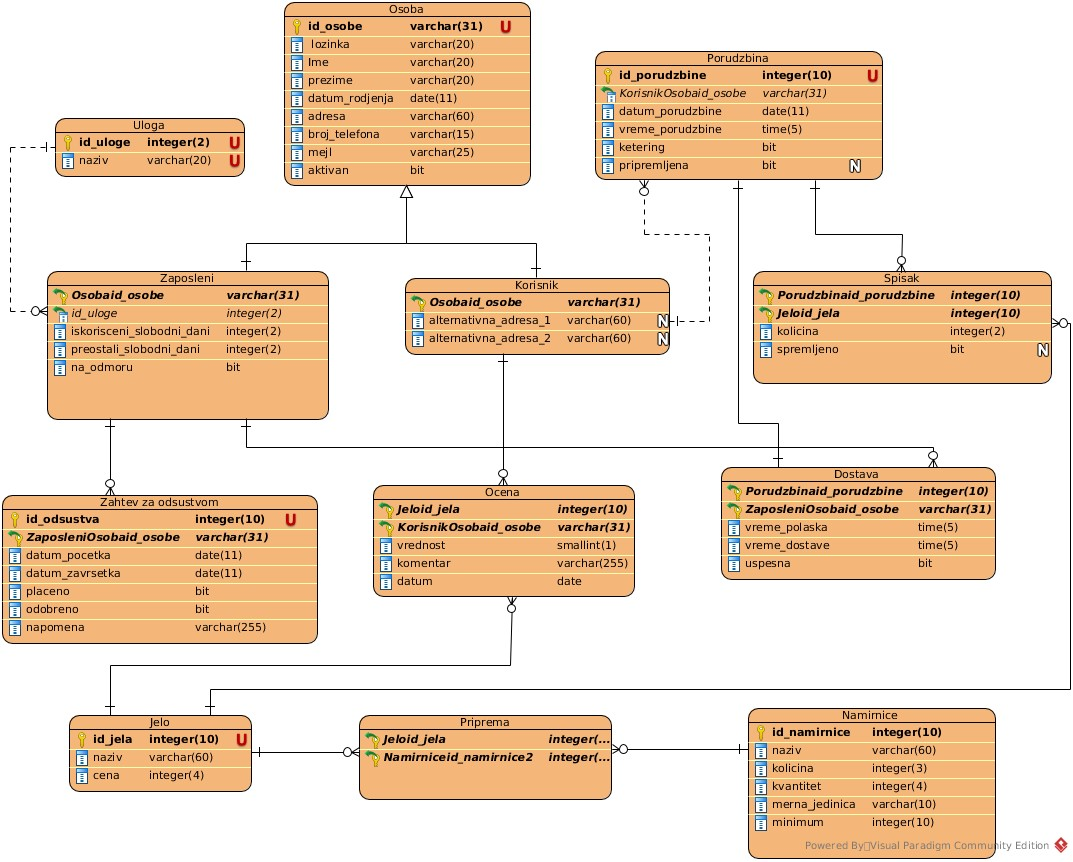
\includegraphics[width=1.1\textwidth]{slike/Baza.jpg}
    \end{center}
    \caption{Dijagram baze podataka}
    \label{fig:slika11}
\end{figure}
\leavevmode
